%遷移金属
\part{遷移金属}
 d軌道・f軌道(内殻)の秋に電子が入っていき、最外殻電子の数は\hl{1か2}\\
 (\hl{ランタノイド}・\hl{アクチノイド}:f軌道に入っていく過程)\\
 同族元素だけでなく、同周期元素も性質が似ている。
 \begin{itemize}
  \item 単体は密度が\hl{大き}く、融点が\hl{高い}金属
  \item d軌道の一部の電子も価電子
  \item 化合物やイオンは\hl{白}色のものが多い
  \item 安定な\hl{錯イオン}を形成しやすい(\hl{d軌道に空きがある})
  \item 単体や化合物は\hl{触媒}になるものが多い\footnote{\R \ce{VsO5,MnO2,Fe3O4,Pt}}
  \item 酸化数が$\left\{\begin{tabular}{l}
  小さい\\大きい
  \end{tabular}\right\}$酸化物は$\left\{\begin{tabular}{l}
  \hl{還元}\\ \hl{酸化}
  \end{tabular}\right\}$剤
 \end{itemize}
 \section{鉄・コバルト・ニッケル}
 \subsection{鉄}
 \subsubsection{性質}
 \begin{itemize}
  \item 常温で\hl{強磁}性
  \item イオン化傾向が水素より\hl{大き}い\\
  \hl{強酸}と反応(\hl{濃硝酸}には\hl{不動態}となり反応しない)
  \item \hl{高温の水蒸気}と反応して\hl{緻密}な\hl{黒錆}が生成(酸化被膜)
  \item 湿った空気中では\hl{粗}い\hl{赤錆}を生成
 \end{itemize}
 \begin{tabular}{|l|l|c|c|}\hline
 酸化鉄(\ajRoman{3})&\ce{Fe2O3}&\hl{赤褐}色&\hl{常磁}性 \\ \hline
 四酸化三鉄&\ce{Fe3O4}&\hl{黒}色&\hl{強磁}性 \\ \hline
 酸化鉄(\ajRoman{2})&\ce{FeO}&\hl{黒}色&\hl{発火}性 \\ \hline
 \end{tabular}\\\\
 \begin{tabular}{|c|c|c|c|c|}\hline
 軟鋼&\hl{鉄鋼}&\hl{銑鉄}&\hl{ステンレス鋼}&KS磁石鋼\\ \hline
 C0.2\% 未満&C2\% 未満&C2\% 以上&\hl{\ce{Cr,Ni}}&\ce{Co,W,Cr}\\ \hline
 加工しやすい&硬くて弾性あり&硬くてもろい&錆びにくい&--- \\ \hline
 鉄筋・鉄骨&レール・バネ&鋳物&キッチン&人工永久磁石\\ \hline
 \end{tabular}
 \newpage
 \subsubsection{製法}
 鉄の製錬 \K\\\\
 \tikz[remember picture,baseline=(kouro.base)] \node[draw=black, rectangle, rounded corners=2pt, line width=1pt, inner sep=5pt, outer sep=0pt, right] (kouro) {\hl{高炉}};\hl{鉄鉱石}(赤鉄鉱\hl{\ce{Fe2O3}}・磁鉄鉱\hl{\ce{Fe2O3}}・不純物)・\hl{コークス}・\hl{石灰石}を高温で反応\par
\begin{quotation}
\hl{\ce{Fe2O3}}
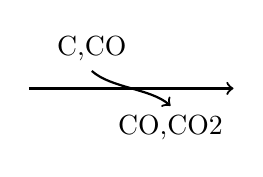
\begin{tikzpicture}[baseline=(base.center)]
\coordinate (base) at (0,-0.1);
\draw[->,thick] (-0.3,0)--(2.3,0);
\node (from) at (0.5,0.5){\hl{\ce{C,CO}}};
\node (to) at (1.5,-0.5){\hl{\ce{CO,CO2}}};
\draw[->,thick] (from.south)..controls (0.75,0) and (1.25,0)..(to.north);
\end{tikzpicture}
\hl{\ce{Fe3O4}}
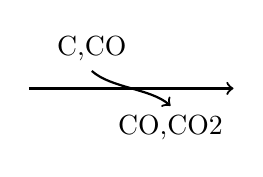
\begin{tikzpicture}[baseline=(base.center)]
\coordinate (base) at (0,-0.1);
\draw[->,thick] (-0.3,0)--(2.3,0);
\node (from) at (0.5,0.5){\hl{\ce{C,CO}}};
\node (to) at (1.5,-0.5){\hl{\ce{CO,CO2}}};
\draw[->,thick] (from.south)..controls (0.75,0) and (1.25,0)..(to.north);
\end{tikzpicture}
\hl{\ce{FeO}}
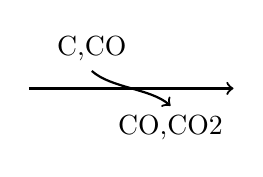
\begin{tikzpicture}[baseline=(base.center)]
\coordinate (base) at (0,-0.1);
\draw[->,thick] (-0.3,0)--(2.3,0);
\node (from) at (0.5,0.5){\hl{\ce{C,CO}}};
\node (to) at (1.5,-0.5){\hl{\ce{CO,CO2}}};
\draw[->,thick] (from.south)..controls (0.75,0) and (1.25,0)..(to.north);
\end{tikzpicture}
\hl{\ce{Fe}}(\hl{銑鉄})
\begin{enumerate}
\item 一酸化炭素の再生\\
\hce{C + CO2 -> 2CO}
\item 石灰石の強熱\\
\hce{CaCO3 -> CaO + CO2}
\item \hl{スラグ}の生成\\
$\left.\begin{tabular}{l}
\hce{CaO + SiO2 -> CaSiO3}\\
\ce{CaO +Al2O3 -> Ca(AlO2)2}
\end{tabular} \right\}$セメントの原料など
\end{enumerate}
\end{quotation}
\begin{tikzpicture}[remember picture, baseline=(tenro.base)]
 \node[draw=black, rectangle, rounded corners=2pt, line width=1pt, inner sep=5pt, outer sep=0pt, right] (tenro) {\hl{転炉}};
 \draw[-latex,very thick,overlay] (kouro.south)--(tenro.north);
\end{tikzpicture}
 \hl{銑鉄}に高温の\hl{酸素}を吹き付けて\hl{鋼}になる。
 \subsubsection{反応}
 \begin{itemize}
  \item 塩酸との反応\\
  \hce{Fe + 2HCl -> FeCl2 + H2 ^}
  \item 高温の水蒸気との反応\\
  \hce{3Fe + 4H2O -> Fe3O4 + 4H2 ^}
  \item 微量に含まれる炭素・鉄・水による\hl{局部電池}(\hl{食塩}などが溶けていたら反応速度上昇)\\
  \begin{tabular}{ll}
  正極(\hl{\ce{C}})&\hce{O2 + 2H2O + 4e- -> 4OH-}\\
  負極(\hl{\ce{Fe}})&\hce{Fe -> Fe^{2+} + 2e-}
  \end{tabular}
  \item \hl{水酸化鉄(\ajRoman{2})}の生成\\
  \hce{Fe^{2+} + 2OH- -> Fe(OH)2}(\hl{緑}色)
  \item 速やかに\hl{水酸化鉄(\ajRoman{2})}が酸素により酸化\\
  \hce{4Fe(OH)2 + O2 + 2H2O -> 4Fe(OH)3}
  \item \hl{水酸化鉄(\ajRoman{3})}の脱水\\
  \ce{Fe(OH)3 -> FeO(OH) + H2O}(酸化水酸化鉄(\ajRoman{3})濃橙色)\\
  \ce{2Fe(OH)3 -> Fe2O3*$n$H2O + $(3-n)$H2O} (\hl{赤褐}色)\\
  (エバンスの実験)
 \end{itemize}
 \subsection{硫酸鉄(\UTF{2161})7水和物}
 化学式:\hl{\ce{FeSO4*7H2O}}
 \subsubsection{性質}
 \begin{itemize}
  \item \hl{青緑}色の固体
  \item \ce{Fe^{2+}}半反応式\\
  \hce{Fe^{2+} -> Fe^{3+} + e-}
  \item 空気中で表面が\hl{\ce{Fe2(SO4)3}}(\hl{黄褐}色)
 \end{itemize}
 \subsubsection{製法}
 鉄に\hl{希硫酸}を加えて、蒸発濃縮\\
 \hce{Fe + H2SO4 -> FeSO4 + H2 ^}
 \subsection{塩化鉄(\UTF{2162})6水和物}
 化学式:\hl{\ce{FeCl3*6H2O}}
 \subsubsection{性質}
 \begin{itemize}
  \item \hl{黄褐}色で\hl{潮解}性のある固体
  \item \hl{酸性}\\
  $\left(
   \begin{tabular}{ll}
    \hl{\ce{Fe^{3+} + H2O <=> Fe(OH)^{2+} + H+}}&$K_{1}=6.0\times10^{-3}$ mol/L\\
   \end{tabular}
   \right)$
 \end{itemize}
 \subsubsection{製法}
 鉄に希塩酸を加えてから、塩素を通じる。\\
 \hce{Fe + 2HCl -> FeCl2 + H2 ^}\\
 \hce{2FeCl2 + Cl2 -> 2FeCl3}
 \subsection{鉄イオンの反応}
 \begin{tabular}{|c|c|c|c|c|c|}\cline{2-6}
 \multicolumn{1}{c|}{}&\ce{NaOH}&\ce{K4[Fe(CN)6]}&\ce{K3[Fe(CN)6]}&\ce{H2S}(酸性)&\ce{KSCN}\\ \hline
 \ce{Fe^{2+}}&\hl{\ce{Fe(OH)2 v}}&\ce{Fe2[Fe(CN)6] v}&\ce{KFe[Fe(CN)6]  v}&\hl{変化なし}&\hl{変化なし}\\
 \hl{淡緑}色&\hl{緑白}色&\hl{青白}色&\hl{濃青}色&\hl{淡緑}色&\hl{淡緑}色\\ \hline
 \ce{Fe^{3+}}&\hl{\ce{Fe(OH)3 v}}&\ce{KFe[Fe(CN)6] v}&\ce{Fe[Fe(CN)6]aq}&\hl{\ce{Fe^{2+}aq}}&\ce{[Fe(NCS)]^{2+}}\\
 \hl{黄褐}色&\hl{赤褐}色&\hl{濃青}色&\hl{暗褐}色&\hl{淡緑}色&\hl{血赤}色\\ \hline
 \end{tabular}
 \begin{itemize}
 \item \ce{Fe^2+,Fe^3+}は、\hl{\ce{OH-}}とも\hl{\ce{NH3}}とも錯イオンを形成しない
 \item ベルリンブルーとターンブルブルーは\hl{同一物質}
 \end{itemize}
 \subsection{塩化コバルト(\UTF{2161})}
 化学式:\hl{\ce{CoCl2}}
 \subsubsection{性質}
 \begin{itemize}
  \item \hl{青}色で\hl{潮解}性のある固体
  \item 6水和物は\hl{淡赤}色
  \item 塩化コバルト紙を用いた\hl{水}の検出
  \item \ce{CO^3+}は\hl{\ce{NH3}}と錯イオンを形成
 \end{itemize}
 \subsection{硫酸ニッケル(\UTF{2161})}
 化学式:\hl{\ce{NiSO4}}
 \begin{itemize}
  \item 黄緑色で潮解性のある固体
  \item 6水和物は青緑色
  \item \ce{Ni^2+}は\hl{\ce{NH3}}と錯イオンを形成
 \end{itemize}
 \section{銅}
 \subsection{銅}
 \subsubsection{性質}
 \begin{itemize}
  \item \hl{赤}色の金属光沢
  \item 他の金属とさまざまな色の\hl{合金}
  \item 展性・延性が\hl{大き}く、電気・熱伝導性が\hl{高}い
  \item イオン化傾向が水素より\hl{低}く、酸化力のある酸と反応\\
  \item 空気中で徐々に酸化して、緻密な錆(\hl{酸}に溶解)が生成\\
  \hl{赤}色の酸化銅(\ajRoman{1})\stamp{Cyan}{乾}・\hl{青緑}色の錆(\hl{緑青})\stamp{RoyalBlue}{湿}
 \end{itemize}
 \subsubsection{製法}
 銅の製錬 \stamp{Sepia}{粗銅}・\hl{電解精錬} \stamp{Maroon}{純銅} \K\\
 \tikz[remember picture,baseline=(kouro1.base)] \node[draw=black, rectangle, rounded corners=2pt, line width=1pt, inner sep=5pt, outer sep=0pt, right] (kouro1) {\hl{高炉}};\hl{黄銅鉱}(\hl{\ce{CuFeS2}})・\hl{コークス}・\hl{石灰石}・\hl{ケイ砂}を高温で反応\par
\begin{quotation}
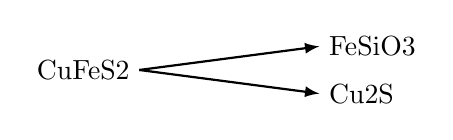
\begin{tikzpicture}
\node (from) at (0,0){\hl{\ce{CuFeS2}}};
\node[right] (to1) at (3,0.3){\ce{FeSiO3}};
\node[right] (to2) at (3,-0.3){\ce{Cu2S}};
\draw[-latex,thick] (from.east)--(to1.west);
\draw[-latex,thick] (from.east)--(to2.west);
\end{tikzpicture}
\end{quotation}
\begin{tikzpicture}[remember picture, baseline=(tenro.base)]
 \node[draw=black, rectangle, rounded corners=2pt, line width=1pt, inner sep=5pt, outer sep=0pt, right] (tenro) {\hl{転炉}};
 \draw[-latex,very thick,overlay] (kouro1.south)--(tenro.north);
\end{tikzpicture}
硫化銅(\ajRoman{1})に\hl{酸素}を吹き付けて、\hl{粗銅}にする。
\begin{quotation}
\ce{2Cu2S + 3O2 -> 2Cu2O + 2SO2}\par
\ce{Cu2S + 2Cu2O -> 6Cu + SO2}
\end{quotation}
 \subsubsection{反応}
 \begin{itemize}
  \item 銅と希硝酸\\
  \hce{3Cu + 8HNO3 -> 3 Cu(NO3)2 + 4H2O + 2NO ^}
  \item 銅と濃硝酸\\
  \hce{Cu + 4HNO3 -> Cu(NO3)2 + 2H2O + 2NO2 ^}
  \item 銅と熱濃硫酸\\
  \hce{Cu + 2 H2SO4 -> CuSO4 + 2H2O + SO2 ^}
  \item 空気中で$1000^\circ$C未満で加熱して、\hl{黒}色の\hl{酸化銅(\ajRoman{2})}生成\\
  \hce{2Cu + O2 -> 2CuO}
  \item さらに$1000^\circ$C以上で加熱して、\hl{赤}色の\hl{酸化銅(\ajRoman{1})}生成\\
  \hce{4CuO -> 2Cu2O + O2}
  \item 銅イオンから水酸化銅(\ajRoman{2})の生成\\
  \hce{Cu2+ + 2OH- -> Cu(OH)2 v}
  \item 水酸化銅(\ajRoman{2})とアンモニアの反応\\
  \hce{Cu(OH)2 + 4NH3 -> [Cu(NH3)4]^{2+} + 2OH-}
  \item 水酸化銅(\ajRoman{2})の加熱\\
  \hce{Cu(OH)2 -> CuO + H2O}
 \end{itemize}
 \subsection{硫酸銅(\UTF{2161})5水和物}
 \subsubsection{性質}
 \begin{itemize}
  \item \hl{青}色の固体(結晶中の\hl{\ce{[Cu(H2O)4]^{2+}}}の色)
  \item 温度による物質変化\\
  \begin{tikzpicture}
  \node (5) at (0,0){5水和物};
  \node (3) at (3,0){\hl{3水和物}};
  \node (1) at (6,0){\hl{1水和物}};
  \node (0) at (9,0){\hl{無水和物}};
  \node (fin) at (12,0){\hl{酸化銅(\ajRoman{2})}};
  \draw[->,thick] (5.east)--node[auto=left] {$102^\circ$C}(3.west);
  \draw[->,thick] (3.east)--node[auto=left] {$113^\circ$C}(1.west);
  \draw[->,thick] (1.east)--node[auto=left] {$150^\circ$C}(0.west);
  \draw[->,thick] (0.east)--node[auto=left] {$650^\circ$C}(fin.west);
  \node (blue) at ([yshift=-5pt]5.south){\hl{青}色};
  \node (white) at ([yshift=-5pt]0.south){\hl{白}色};
  \draw[<-,thick] (blue.east)--node[auto=right] {+\ce{H2O}(検出)}(white.west);
  \end{tikzpicture}
  \item \ce{Cu^2+}による\hl{殺菌}作用(農薬)
  \item 還元性を持つ有機化合物の検出\footnote{フェーリング液・ベネディクト液}\\
  \hl{赤}色の酸化銅(\ajRoman{1})が生成
 \end{itemize}
 \subsubsection{製法}
 銅に\hl{濃硫酸}をかけてから\hl{加熱}。
 \subsection{銅(\UTF{2161})イオンの反応}
 \begin{tabular}{|c|c|c|c|c|}\cline{2-5}
 \multicolumn{1}{c|}{}&少々の塩基&過剰の\ce{NH3}&濃塩酸&\ce{H2S}(\hl{全液性})\\ \hline
 \ce{Cu^{2+}}&\hl{\ce{Ca(OH)2 v}}&\hl{\ce{[Ca(NH3)4]^{2+} aq}}&\hl{\ce{[CuCl4]^{2-} aq}}&\hl{\ce{CuS v}}\\
\hl{青}色&\hl{青白}色&\hl{深青}色&\hl{黄緑}色&\hl{黒}色\\ \hline
 \end{tabular}
 \begin{itemize}
  \item 炎色反応:\hl{青緑}色
  \item 加熱すると\hl{分解}
  \item \ce{Cu^2+}は\hl{\ce{NH3}}と錯イオンを形成し、\hl{\ce{OH-}}とは形成しない
 \end{itemize}
 \subsection{銅の合金}
 \begin{tabular}{|c|c|c|c|c|}\hline
 \hl{黄銅}(真鍮)&\hl{洋銀}(洋白)&\hl{白銅}&\hl{青銅}&\hl{ジュラルミン}\\ \hline
 \hl{\ce{Zn}}&\hl{\ce{Zn,Ni}}&\hl{\ce{Ni}}&\hl{\ce{Sn}}&\hl{\ce{Al}}(主成分)\\ \hline
 適度な強度と加工性&柔軟で錆びにくい&柔軟で錆びにくい&硬くて錆びにくい&軽くて丈夫\\
 楽器・水道用具&食器・装飾品&五十円玉・五百円玉&像&航空機・車両\\ \hline
 \end{tabular}
 \section{銀}
 \subsection{銀}
 \subsubsection{性質}
 \begin{itemize}
  \item 展性・延性が\hl{大きく}、電気・熱伝導性が\hl{最も高い}
  \item イオン化傾向が水素より\hl{小さい}\\
  \hl{酸化}力のある酸(\hl{硝酸}・\hl{熱濃硫酸})と反応
  \item 空気中で酸化しにくいが、\hl{硫化水素}とは容易に反応
 \end{itemize}
 \subsubsection{製法}
  \begin{itemize}
  \item 銅の電解精錬の\hl{陽極泥} \K
  \item 銀の化合物の熱分解・光分解\\
  酸化銀の熱分解\\
  \hce{2Ag2O -> 4Ag + O2}\\
  ハロゲン化銀\ce{AgX}の感光\\
  \hce{2AgX -> 2Ag + X2}
 \end{itemize}
 \subsubsection{反応}
 \begin{itemize}
  \item 銀と希硝酸\\
  \hce{3Ag + 4HNO3 -> 3AgNO3 + 2H2O + NO ^}
  \item 銀と濃硝酸\\
  \hce{Ag + 2HNO3 -> AgNO3 + H2O + NO2 ^}
  \item 銀と熱濃硫酸\\
  \hce{2Ag + 2H2SO4 -> Ag2SO4 + 2 H2O + SO2 ^}
  \item 銀と硫化水素\\
  \hce{4Ag + 2H2S + O2 -> 2Ag2S + 2H2O} 
 \end{itemize}
 \subsection{銀(\UTF{2160})イオンの反応}
 \hl{硝酸銀}水溶液\\
 \begin{tabular}{|c|c|c|c|c|c|}\cline{2-6}
 \multicolumn{1}{c|}{}&少量の塩基&過剰の\ce{NH3}&\ce{HCl}&\ce{H2S}(\hl{全液}性)&\ce{K2CrO4}\\ \hline
 \ce{Ag^2+}&\hl{\ce{Ag2O v}}&\hl{\ce{[Ag(NH3)2]+}}&\hl{\ce{AgCl v}}&\hl{\ce{Ag2S v}}&\hl{\ce{Ag2CrO4 v}}\\
 \hl{無}色&\hl{褐}色&\hl{無}色&\hl{白}色&\hl{黒}色&\hl{赤褐}色\\ \hline
 \end{tabular}
 \begin{itemize}
  \item 銀と少量の塩基\\
  \hce{2Ag+ + 2OH- -> Ag2O v + H2O}
  \item 銀と過剰の\ce{NH3}\\
  \hce{Ag2O + 4NH3 + H2O -> 2[Ag(NH3)2]+ + 2OH-}
  \item 銀と\ce{HCl}\\
  \hce{Ag+ + Cl- -> AgCl v}
  \item 銀と\ce{H2S}\\
  \hce{2Ag+ + S2- -> Ag2S v}
  \item 銀と\ce{K2CrO4}\\
  \hce{AgCl + 2 NH3 -> [Ag(NH3)2]+ + Cl-}
 \end{itemize}
 \subsection{難溶性化合物の溶解性}
 \begin{tabular}{|cr|c|c|c|c|}\cline{3-6}
 \multicolumn{2}{c|}{}&\ce{HNO3}&\ce{NH3}&\ce{NaS2O3}&\ce{KCN}\\ \hline
 \ce{Ag2S v}&\hl{黒}色&\hl{溶ける}&\hl{溶けない}&\hl{溶けない}&\hl{溶ける}\\ \hline
 \ce{Ag2O v}&\hl{褐}色&\hl{溶ける}&\hl{溶ける}&\hl{溶ける}&\hl{溶ける}\\ \hline
 \ce{AgCl v}&\hl{白}色&\hl{溶けない}&\hl{溶ける}&\hl{溶ける}&\hl{溶ける}\\ \hline
 \ce{AgBr v}&\hl{淡黄}色&\hl{溶けない}&\hl{やや溶ける}&\hl{溶ける}&\hl{溶ける}\\ \hline
 \ce{AgI v}&\hl{黄}色&\hl{溶けない}&\hl{溶けない}&\hl{溶ける}&\hl{溶ける}\\ \hline
 溶解している物質&\hl{無}色&\hl{\ce{Ag+(AgNO3)}}&\hl{\ce{[Ag(NH3)2]+}}&\hl{\ce{[Ag(S2O3)2]^3-}}&\hl{\ce{[Ag(CN)2]-}}\\ \hline
 \end{tabular}
 \newpage
 \section{クロム・マンガン}
 化学式:\hl{\ce{Cr}}・\hl{\ce{Mn}}
 \subsection{単体}
 \subsubsection{性質}
 \begin{itemize}
  \item \hl{強酸}と反応(\hl{\ce{Cr}}は\hl{濃硝酸}には\hl{不動態}となり反応しない)
  \item 空気中で錆び\hl{にくい}(\hl{不動態})$\Rightarrow$\hl{ステンレス鋼}(\ce{Fe,Cr,Ni})\stamp{teal}{クロム}\\
  空気中で錆び\hl{やすい} \stamp{teal}{マンガン}
  \item \hl{ニクロム}合金(\ce{Fe,Cr,Mn})(電熱線・発熱体)
 \end{itemize}
 \subsubsection{反応}
 \begin{itemize}
  \item クロムと希塩酸\\
  \hce{Cr + 2HCl -> CrCl2 + H2 ^}(\ce{Cr^2+}:青色)
  \item マンガンと希塩酸\\
  \hce{Mn + 2HCl -> MnCl2 + H2 ^}(\ce{Mn^2+}:\hl{淡桃}色)
 \end{itemize}
 \subsection{クロム酸カリウム・二クロム酸カリウム}
 化学式:\hl{\ce{K2CrO4}}・\hl{\ce{K2Cr2O7}}
 \subsubsection{性質}
 \begin{itemize}
  \item 二つは平衡状態にある\\
  \begin{tabular}[h]{ccc}
  \hl{\ce{2CrO4^{2-} + H+}}&\ce{<=>}&\hl{\ce{Cr2O7^{2-} + OH-}}\\
  \hl{塩基}性・\hl{黄}色&&\hl{酸}性・\hl{赤橙}色
  \end{tabular}
  \item \hl{酸化}剤として反応 \stamp{teal}{二クロム酸カリウム}\\
  \hce{Cr2O7^{2-} + 14H+ + 6e- -> 2Cr^{3+} + 7H2O}(\hl{硫酸酸性}下)
 \end{itemize}
 \subsubsection{製法}
 \begin{enumerate}
  \item クロム(\ajRoman{3})イオンに少量の水酸化ナトリウム水溶液を加える\\
  \hce{Cr^3 + 3OH- -> Cr(OH)3 v}
  \item さらに水酸化ナトリウム水溶液を加える(過剰の水酸化ナトリウム水溶液を加える)\\
  \hce{Cr(OH)3 + OH- -> [Cr(OH)4]-}
  \item 過酸化水素水を加えて加熱\\
  \hce{2[Cr(OH)4]- + 3H2O2 + 2OH- -> 2CrO4^{2-} + 8H2O}
 \end{enumerate}
 \subsubsection{反応}
 \begin{itemize}
  \item クロム酸イオンと銀イオン\\
  \hce{CrO4^{2-} + 2Ag+ -> Ag2CrO4 v}(\hl{赤褐}色)
  \item クロム酸イオンと銀イオン\\
  \hce{CrO4^{2-} + Ba^{2+} -> BaCrO4 v}(\hl{黄}色)
  \item クロム酸イオンと銀イオン\\
  \hce{CrO4^{2-} + Ag^{2+} ->PbCrO4}(\hl{黄}色)
 \end{itemize}
 \subsection{過マンガン酸カリウム}
 化学式:\hl{\ce{KMnO4}}
 \subsubsection{性質}
 \begin{itemize}
  \item \hl{黒紫}色の固体
  \item \hl{酸化}剤として反応\\
  \begin{tabular}{cl}
  \hl{硫酸}酸性&\hce{MnO4- + 8H+ + 5e- -> Mn^2+ + 4H2O}\\
  中・塩基性&\hce{MnO4- + 2H2O + 3e- -> MnO2 + 4OH-}
  \end{tabular}
 \end{itemize}
 \subsubsection{製法}
 \begin{enumerate}
  \item 酸化マンガン(\ajRoman{4})と水酸化ナトリウムを混ぜて空気中で加熱\\
  \hce{2MnO2 + 4KOH + O2 -> 2K2MnO4 + 2H2O}(\ce{MnO2}:\hl{黒褐}色/\ce{K2MnO4}:\hl{緑}色)
  \item
  \begin{enumerate}
  \item 酸性にする\\
  \hce{3MnO4^{2-} + 4H+ -> 2MnO4- + MnO2 + 2H2O}(\ce{MnO4^{2-}}:\hl{緑}色/\ce{MnO4-}:\hl{赤紫}色)
  \item 電気分解する\\
  (\hl{陽}極)\hce{MnO4^{2-} -> MnO4^- + e-}
  \end{enumerate}
 \end{enumerate}
 \subsection{マンガンの安定な酸化数}
 残留酸素の定量(ウィンクラー法)
 \begin{enumerate}
  \item マンガン(\ajRoman{3})イオンを含む水溶液に塩基を加える\\
  \hce{Mn^2+ + 2OH- -> Mn(OH)2 v}
  \item 水酸化マンガン(\ajRoman{2})が水溶液中の溶存酸素と速やかに反応\\
  \hce{2Mn(OH)2 + O2 -> 2MnO(OH)2}
  \item 希硫酸を加える\\
  \hce{MnO(OH)2 + 4H+ + 2e- -> Mn^2+ + 3H2O}(\hl{酸化}剤)
 \end{enumerate}